\documentclass[11pt,aspectratio=43]{beamer}
\usepackage[utf8]{inputenc}
\usepackage{amsmath, amsfonts, amssymb, amsthm}
\usepackage[T1]{fontenc}
\usepackage{lmodern}
\usepackage{xcolor}
\usepackage{setspace}
\usepackage{booktabs}
\usepackage{multirow}
\usepackage{graphicx}
\usepackage{tikz}
% \usetikzlibrary{decorations}
\usetikzlibrary{decorations.pathreplacing}
\usepackage{ulem}
\usepackage{hyperref}
\usepackage{booktabs}
\usepackage{babel}
\usepackage{makecell}
\usepackage[para,online,flushleft]{threeparttable}
\usepackage{pdfpages}
\usepackage{tcolorbox}
\usepackage{bm}
\usepackage{appendixnumberbeamer}
\usepackage{natbib}
\usepackage{caption}
\captionsetup[figure]{labelformat=empty}% redefines the caption setup of the figures environment in the beamer class.
\usetheme[compress]{Boadilla}
\usecolortheme{default}
\useoutertheme{miniframes}
\usefonttheme[onlymath]{serif}

\newcommand{\jump}[2]{\hyperlink{#1}{\beamerbutton{#2}}}
\newcommand{\orange}[1]{\textcolor{orange}{#1}}
\newcommand{\red}[1]{\textcolor{red}{#1}}

\setbeamertemplate{itemize item}{\raisebox{0.1em}{\scalebox{0.7}{$\blacksquare$}}}
\setbeamertemplate{itemize subitem}[circle]
\setbeamertemplate{itemize subsubitem}{--}
\setbeamercolor{itemize item}{fg=black}
\setbeamercolor{itemize subitem}{fg=black}
\setbeamercolor{itemize subsubitem}{fg=black}
\setbeamercolor{item projected}{bg=darkgray,fg=white}
\definecolor{blue}{rgb}{0.2, 0.2, 0.7}
\setbeamercolor{alerted text}{fg=blue}
\setbeamertemplate{enumerate items}[circle]


\setbeamertemplate{headline}{}

%==========================================
\let\olditemize=\itemize
\let\endolditemize=\enditemize
\renewenvironment{itemize}{\olditemize \itemsep1em}{\endolditemize}
\let\oldenumerate=\enumerate
\let\endoldenumerate=\endenumerate
\renewenvironment{enumerate}{\oldenumerate \itemsep1em}{ \endoldenumerate}

\DeclareMathOperator*{\argmax}{\arg\!\max}
\DeclareMathOperator*{\E}{\mathbb{E}}
\DeclareMathOperator*{\var}{\rm Var}
\DeclareMathOperator*{\cov}{\rm Cov}

\theoremstyle{definition}
\newtheorem{assume}{Assumption}
\newtheorem{lem}{Lemma}
\newtheorem{proposition}{Proposition}
\newtheorem{thm}{Theorem}
\newtheorem{corol}{Corollary}

\begin{document}
    \title[Lecture 11]{Lecture 11 \\ Distorting Taxes and the Welfare Theorems}
    \author[Hui-Jun Chen]{Hui-Jun Chen}
    \institute[OSU]{The Ohio State University}
    % \date{\today}
    \date{\today}
    \setbeamertemplate{navigation symbols}{}
    \setstretch{1.2}

%-------------------------------------------------------
{
%	\usebackgroundtemplate{\includegraphics[width=1\paperwidth]{../EveningSky_cropped_edit43_bright.jpg}}
    \begin{frame}
% \vspace{3em}
        \centering
%		{\footnotesize 	ECON 4002 Intermediate Macroeconomic Theory}
        \maketitle
% \vspace{-1.5em}
% \centering
% \includegraphics[width=0.55\linewidth]{Pictures/houses.jpeg}


    \end{frame}
}

% -------------------------------------------
\setbeamertemplate{headline}
{
\setbeamercolor{section in head/foot}{fg=black, bg=white}
\vskip1em \tiny \insertsectionnavigationhorizontal{1\paperwidth}{\hspace{0.50\paperwidth}}{}
}
%------------------------------------------

\begin{frame}{Overview}
\label{slide:Overview}

In previous lectures, all the taxes we are discussing is \alert{lump-sum tax}.

\begin{itemize}
    \item pure \alert{income effect}, no change to consumption-leisure allocation
    \item satisfy both welfare theorems
\end{itemize}

In this lecture, the \alert{distorting taxes} will include \alert{substitution effect}, and thus

\begin{itemize}
    \item creating ``wedges'' to distort consumption-leisure choice
    \item violate the welfare theorems (CE $ \neq $ SPP)
\end{itemize}

\end{frame}

\section{Simplified Model}
\label{sec:Simplified_Model}

\begin{frame}{SPP in Simplified Model}
\label{slide:SPP_in_Simplified_Model}
    \begin{columns}
        \begin{column}{0.5\textwidth}
            \begin{figure}
                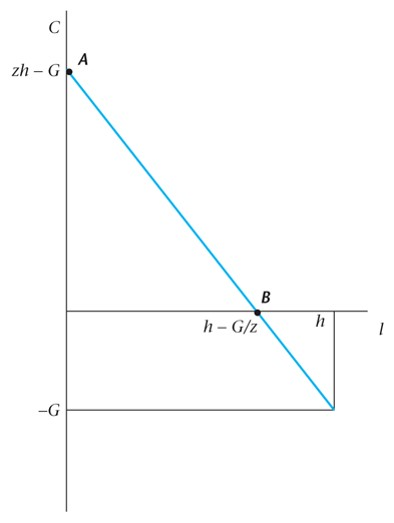
\includegraphics[width=\textwidth]{./figures/Figure_5_14.jpg}
            \end{figure}
        \end{column}
        \begin{column}{0.5\textwidth}
            Assume production is labor-only technology:

            %
            \begin{equation*}
               Y = z N^{d}
            \end{equation*}
            %
            So PPF is
            %
            %
            \begin{equation*}
               C = z( h-l ) - G
            \end{equation*}
            %
            Thus, SPP is
            %
            \begin{align*}
                    & \max_{l} U( z( h-l ) - G, l )
                \\
                \text{FOC:} \quad
                    & \frac{D_{l}U( C, l )}{D_{C}U( C, l )} = MRS_{l, C}
                \\
                    & = MRT_{l, C} = z = MPN
            \end{align*}
            %
        \end{column}
    \end{columns}
\end{frame}

\begin{frame}{Labor Demand in Simplified Model}
\label{slide:Labor_Demand_in_Simplified_Model}
    \begin{columns}
        \begin{column}{0.5\textwidth}
            \begin{figure}
                \caption{\scriptsize Figure 5.15  The Labor Demand Curve in the Simplified Model}
                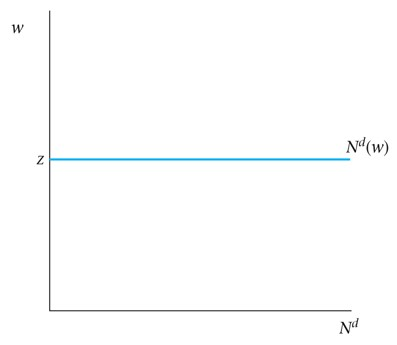
\includegraphics[width=\textwidth]{./figures/Figure_5_15.jpg}
            \end{figure}
        \end{column}
        \begin{column}{0.5\textwidth}
            %
            \begin{equation*}
                 \max_{N^{d}} z N^{d} - wN^{d}
            \end{equation*}
            %
            FOC would be $ z = w $ (horizontal line)
            \begin{itemize}
                \item if $ z < w $: negative profit for every worker hired, choose $ N^{d} = 0 $
                \item if $ z > w $: positive profit for every worker hired, choose $ N^{d} = \infty $
                \item only $ z = w $ possible, $ \therefore $ linear PPF in previous slide
                \begin{itemize}
                    \item ``infinitely elastic'' $ N^{d} $
                \end{itemize}
            \end{itemize}
        \end{column}
    \end{columns}
\end{frame}

\begin{frame}{Competitive Equilibrium w/ Distorting Tax}
\label{slide:Competitive_Equilibrium_w__Distortionary_Tax}
    A competitive equilibrium, with $ \{ z, \alert{G} \} $ exogenous, is a list of endogenous prices and quantities $ \{ C, l, N^{s}, N^{d}, Y, \pi, w, \alert{t} \} $ such that:
    \begin{enumerate}
        \item  taking $ \{ w, \pi \} $ as given, the consumer solves
        %
        %
        %
        \begin{equation*}
            \max_{C, l, N^{s}} U( C, l )
            \quad \text{subject to} \quad
            C = w\alert{( 1-t )}N^{s} + \pi
            \quad \text{and} \quad
            N^{s} + l = h
        \end{equation*}
        %
        \item taking $ w $ as given, the firm solves:
        %
        \begin{equation*}
            \max_{N^{d}, Y, \pi} \pi
            \quad \text{subject to} \quad
            \pi = Y - w N^{d}
            \quad \text{and} \quad
            Y = z N^{d}
        \end{equation*}
        %
        \item the government spends $ G = w t N^{s} $
        \item the labor market clears at the equilibrium wage, i.e. $ N^{s} = N^{d} $
    \end{enumerate}
\end{frame}

\begin{frame}{Effect of Distorting Tax}
\label{slide:Effect_of_Distorting_Tax}
    Since the tax is imposed on consumers/workers, it distorted the consumption-leisure decision:
    %
    \begin{equation*}
        MRS_{l, C} = w( 1-t )
    \end{equation*}
    %
    So in the equilibrium, it deviates from SPP:
    %
    \begin{equation*}
        MRS_{l, C} = w( 1-t ) < w = z = MPN = MRT_{l, C}
    \end{equation*}
    %
    \textbf{Result}: CE and SPP lead to different allocation!
\end{frame}

\begin{frame}{Graphical Representation}
\label{slide:Graphical_Representation}
    \begin{columns}
        \begin{column}{0.5\textwidth}
            \begin{figure}
                \caption{\scriptsize Figure 5.16  Competitive Equilibrium in the Simplified Model with a Proportional Tax on Labor Income}
                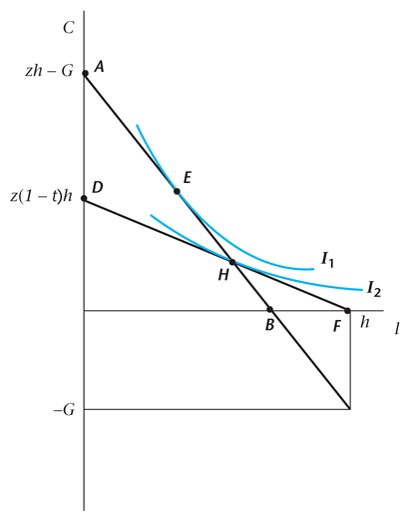
\includegraphics[width=\textwidth]{./figures/Figure_5_16.jpg}
            \end{figure}
        \end{column}
        \begin{column}{0.5\textwidth}
            SPP solution lies at point E:
            \begin{itemize}
                \item $\overline{AB}$: PPF, slope  $ -z $
                \item can reach indifference curve $ I_{1} $
            \end{itemize}
            CE solution lies at point H:
            \begin{itemize}
                \item $\overline{DF}$: consumer’s budget line
                \item can only reach $ I_{2} $
                \item proportional tax $ \Rightarrow  $ $ N^{s} $ $ \downarrow  $
                \item $ N^{s} $$ \downarrow $$ \Rightarrow $$ Y $$\downarrow  $, but still need to meet $ G $, so $ C \downarrow  $: gov’t budget critical!
            \end{itemize}
        \end{column}
    \end{columns}
\end{frame}

\section{Full Model}
\label{sec:Full_Model}

\begin{frame}{How Much Tax Revenue can be Generated?}
\label{slide:How_Much_Tax_Revenue_can_be_Generated_}
    \begin{columns}
        \begin{column}{0.5\textwidth}
            \begin{figure}
                \caption{\scriptsize Figure 5.17  A Laffer Curve}
                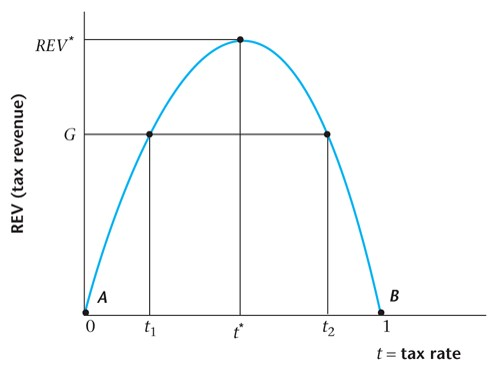
\includegraphics[width=\textwidth]{./figures/Figure_5_17.jpg}
            \end{figure}
            \jump{slide:Multiple_Competitive_Equilibria_Possible}{Back}
        \end{column}
        \begin{column}{0.5\textwidth}
            \small
            equilibrium wage: $ w = z $, implies \alert{total tax revenue} by solve consumer problem:
            %
            \begin{equation*}
                R( t ) = tz( h - l^{*}( t ) )
            ,\end{equation*}
            %
            What $ t $ maximizes? Solve
            %
            \begin{equation*}
               \max_{t} R( t ) = \max_{t} tz( h - l^{*}( t ) )
            ,\end{equation*}
            %
            \begin{itemize}
                \item not just $ t = 1 $! tax \alert{rate } vs tax \alert{base}
                \item $ t = 0 $: no revenue because no tax
                \item $ t = 1 $: no revenue because no incentive to work
            \end{itemize}
        \end{column}
    \end{columns}
\end{frame}

\begin{frame}{Full Model Elaboration}
\label{slide:Full_Model_Elaboration}
    Let $ U( C, l ) = \ln C + \ln l $, and $ h = z = 1 $, by firm's problem we know $ w = z = 1 $.
    Consumer has some non-labor income denoted as $ x > 0 $. FOC leads to
    %
    \begin{align*}
        MRS_{l, C}
            & = \frac{C}{l}
        \\
            & = \frac{( 1-t )( 1-l ) + \pi}{l} = 1 - t < 1 = MRT_{l, C}
        \\
            & \Rightarrow ( 1-t )( 1-l ) + \pi = ( 1-t )l
        \\
            & \Rightarrow 1-l + \frac{\pi}{1-t} = l \Rightarrow 2 l = 1 + \frac{\pi}{(1-t)}
        \\
            & \Rightarrow l = \frac{1}{2} + \frac{\pi}{2(1-t)}
        \\
            & \red{ \Rightarrow N^{s} ( t ) = 1-l = \frac{1}{2} - \frac{\pi}{2(1-t)} }
    \end{align*}
    %
\end{frame}

\begin{frame}{Maximize Tax Revenue}
\label{slide:Maximize_Tax_Revenue}
    Total tax revenue is
    %
    \begin{equation*}
       R( t ) = t N^{s}( t )
    ,\end{equation*}
    %
    and thus government's problem is
    %
    \begin{equation*}
       \max_{t} \frac{1}{2}t - \frac{t\pi}{2(1-t)}
    .\end{equation*}
    %
    FOC leads to
    %
    \begin{align*}
        \frac{1}{2} - \frac{\pi(1-t) + t\pi}{2(1-t)^{2}}
            & = 0 \Rightarrow \frac{1}{2} - \frac{\pi}{2(1-t)^{2}} = 0
        \\
        \frac{1}{2}
            & = \frac{\pi}{2(1-t)^{2}} \Rightarrow 1 = \frac{\pi}{(1-t)^{2}}
        \\
        t
            & = 1 - \sqrt{\pi}
    \end{align*}
    %
\end{frame}

\begin{frame}{Visualization}
\label{slide:Visualization}
    \begin{columns}
        \begin{column}{0.5\textwidth}
            \begin{figure}
                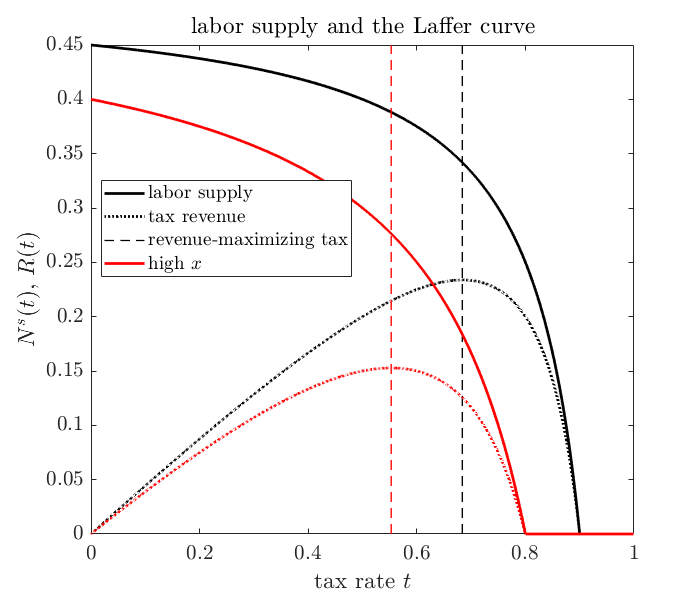
\includegraphics[width=\textwidth]{./figures/lafferCurve.png}
            \end{figure}


        \end{column}
        \begin{column}{0.5\textwidth}
            Consider two cases:
            \begin{enumerate}
                \item consumer is poor (low $ \pi $)
                \item consumer is rich (high $ \pi $)
            \end{enumerate}
            For a given after tax-wage , rich consumer supplies less labor
            \begin{itemize}
                \item tax revenue shifts down
                \item Laffer peak shifts left
                \item many other conditions also impact this analysis!
            \end{itemize}
        \end{column}
    \end{columns}
\end{frame}

\begin{frame}{Multiple Competitive Equilibria Possible}
\label{slide:Multiple_Competitive_Equilibria_Possible}
    \begin{columns}
        \begin{column}{0.5\textwidth}
            \begin{figure}
                \caption{Figure 5.18  Two Competitive Equilibria}
                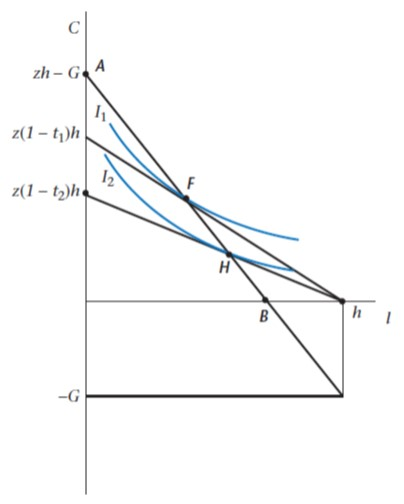
\includegraphics[width=\textwidth]{./figures/Figure_5_18.jpg}
            \end{figure}
        \end{column}
        \begin{column}{0.5\textwidth}
            Previous slide logic implies the government can choose 2 tax rates for a given required level of $ G $
            \begin{itemize}
                \item both $ t_{1} $ and $ t_{2} $ yield the same revenue
                \item consumer strictly better off under lower tax rate $ t_{1} $
            \end{itemize}
            \jump{slide:How_Much_Tax_Revenue_can_be_Generated_}{Tax Revenue}
        \end{column}
    \end{columns}
\end{frame}

\begin{frame}{Conclusion}
\label{slide:Conclusion}
    We’ve focused on the simple case to keep analysis straightforward, but logic applies more broadly.
    \begin{itemize}
        \item SPP: $ MRS_{l, C} = MRT_{l, C} = MPN $, since PPF is $ C = z F( K, N ) - G $
        \item CE: same distortion as our simple case:
        \begin{itemize}
            \item consumer problem implies $ MRS_{l, C} = w ( 1-t ) $
            \item firm problem implies $ MRT_{l, C} = w $
            \item same result as simplified model: $ MRS_{l, C} \neq MRT_{l, C} $, unlike SPP
            \item only difference from simplified model: $ MPN = D_{N}F( K, N ) \neq z $
        \end{itemize}
    \end{itemize}
\end{frame}

\end{document}
